\chapter{Crypto.Types.Elliptic\_Curves}\label{ConceptofElliptic}
For a deeper understanding of the elliptic curves, we provide an
introduction to elliptic curves for convenience of readers before we
continue with the algorithms in Section \ref{EllipticRoot}.

%%%%%%%%%%%%%%%%%%%%%%%%%%%%%%%%%%%%%%%%%%%%%%%%%%%%%%%
%%%%%%%%%%%%%%%%%%%%%%%%%%%%%%%%%%%%%%%%%%%%%%%%%%%%%%%

\section{Mathematical Concept of Elliptic Curves}
\paragraph{Finite Field $F_p^1$.}
For a given prime p, is an algebraic system defined on the number set
$F=\{0,1,\cdots,p-1\}$ with two operations \cite{SimpleTutorial}:

\begin{itemize}
\item Addition: $\forall$ $a,b\in F_p^1$\,, $r\equiv a+b \mod p$\,,
\item Multiplication: $\forall$ $a,b\in F_p^1$\,, $r\equiv a\times b \mod p$\,.
\end{itemize}

\paragraph{Galois Field.} A Galois field ($GF(2^m)$) is a finit field
where each element can be  expressed as a polynomial with degree less than $m$ (
$\forall$ $a \in GF(2^m)$\,,\,$\exists$ $m$ numbers $a_i\in
\{0,1\}$\,,\,$a=a_{m-1}x^{m-1}+\cdots +a_1x+a_0=(a_{m-1}\cdots a_0)$),
and satisfying \cite{SimpleTutorial}:
\begin{itemize}
\item Addition: $\forall$ $a,b\in GF(2^m)$\,, $a+b=c=(c_{m-1}\cdots
  c_0)$\,,\, $c_i=a_i+b_i\mod 2$ = $a_i\oplus b_i$\,,
\item Multiplication: $\forall$ $a,b\in GF(2^m)$\,, $a\times b=c$,
  $c=(\sum_{j=0}^{m-1}a_jx^j)\times (\sum_{j=0}^{m-1}b_jx^j)\mod
  f(x)$, where $f(x)=x^m+\sum_{j=0}^{m-1}f_jx^j$ is an irreducible
  polynomial with degree $m$\,.
\end{itemize}

\paragraph{Characteristic.} of a field $F$, $char(F)$, is the smallest
positive integer of $F$ which satisfies: $\sum_{i=1}^{n}I=0$, where
$I$ is the identity of the field multiplication \cite{SimpleTutorial}.

An elliptic curve $E$ over a finite field $F$ is given by the
Weierstrass equation:
\begin{equation}
  E : y^2 + a_1xy + a_3y = x^3 + a_2x^2 + a_4x + a_6\,, \label{GenerForm}
\end{equation}
where $a_1,a_2,a_3,a_4,a_6$ are coefficients in $F$.

A point ”at infinity” is defined. The Equation \ref{GenerForm} shall
be simplified under assumption about the characteristic of $F$ mapping
$(x,y)$ to $(x',y')$ by invertible linear transformations
\cite{Cohen}. These transformations correspond to morphisms of the
affine part of $E$ to the affine part of another elliptic curve $E'$,
and since the infinite point keeps unchanged an isomorphism between
$E$ and $E'$ is achieved \cite{Cohen}. After all transformations are
done, we change the notation and denote the transformed curve by $E$
with coordinates $(x,y)$ again \cite{Cohen}.\\ Supposed the
characteristic of $F$ is odd. The following transformations are made:
\begin{equation*}
x\mapsto x'\quad\hbox{and}\quad y\mapsto y'= y + \frac{1}{2}(a_1x +a_3)\,,
\end{equation*}
The equation of $E$ is expressed in the coordinates $(x',y')$, then
change notation and write $x$ for $x'$ and $y$ for $y'$, we get:
\begin{equation*}
E:y^2 = x^3 + \frac{b_2}{4}x^2 + \frac{b_4}{2}x + \frac{b_6}{4}\,,
\end{equation*}
where $b_2={a_1}^2+4a_2$\,,\,$b_4=2a_4+a_1a_3$ and
$b_6={a_3}^2+4a_6$\,.\\ Additionally if the characteristic of $F$ is
prime to 6. There goes another transformation:
\begin{equation*}
x\mapsto x'=x+\frac{b_2}{12}\quad\hbox{and}\quad y\mapsto y'\,,
\end{equation*}
and it becomes:
\begin{equation*}
E:y^2 = x^3 - \frac{c_4}{48}x - \frac{c_6}{864}\,,
\end{equation*}
where $c_4$ and $c_6$ are expressed in terms of $b_2,b_4,b_6$ as
\begin{equation*}
c_4={b_2}^2-24b_4\quad\hbox{and}\quad c_6=-{b_2}^2+36b_2b_4-216b_6\,.
\end{equation*}
So if $char(F)$ is prime to 6, Equation (\ref{GenerForm}) can be given
by a short Weierstrass equation of the type:
\begin{equation}
E:y^2 = x^3 + Ax + B\,, \label{SimpleForm}
\end{equation}
where $A,B\in F$.  The discriminant of the curve (\ref{GenerForm}) is
equal to the polynomial discriminant of the curve (\ref{SimpleForm}):
\begin{equation}
\bigtriangleup_{E} = -16(4A^3 + 27B^2)\,.
\end{equation}
A curve is non-singular if and only if the discriminant is unequal to zero.\\ 
 absolute invariant ($j$-invariant) $j_E$ of $E$ is given by
\begin{equation}
j_E = 12^3\frac{-4A^3}{\bigtriangleup_E}\,.\label{Invariant}
\end{equation} \\
If $char(F)=2$ or $3$, $E$ is supersingular if and only if its
$j$-invariant (\ref{Invariant}) is zero \cite{Cohen}.\\ For
$char(F)=2$, in the case of $a_1=0$, Equation (\ref{GenerForm}) can be
transformed to
\begin{equation}\label{Simple2}
E': y^2+Cy=x^3+Ax+B\,,
\end{equation}
where $A,B,C\in K$.\\
While in the case of $a_1\neq 0$, Equation (\ref{GenerForm}) can be transformed to
\begin{equation}\label{Simple3}
E': y^2+xy=x^3+Ax^2+B\,,
\end{equation}
where $A,B\in K$.\\ \ \\ 

\textbf{Group Law on Elliptic Curve: Point Addition and Point
  Doubling} \cite{Cohen}\\ For points $P=(x_1,y_1)$ and $Q=(x_2,y_2)$
on a curve $E$ of the form in Equation \ref{GenerForm}, $P\oplus
Q=(x_3,y_3)$ and\\
\begin{tabular}{llc}
\midrule \quad\quad $-P$ & = & $(x_1,-y_1-a_1x_1-a_3)$,\\ \quad\quad
$P\oplus Q$ & = & \quad\quad$(\lambda^2+a_1\lambda-a_2-x_1-x_2,\quad\lambda(x_1-x_3)-y_1-a_1x_3-a_3)$,\\ \bottomrule
\end{tabular}\\
where
\begin{equation*}
      \lambda =
      \left\{
       \begin{array}{ll}
       \frac{y_2-y_1}{x_2-x_1}\qquad\qquad\quad\quad \hbox{if $P\neq\pm Q$ (point addition)} \\
       \frac{3x_1^2+2a_2x_1+a_4-a_1y_1}{2y_1+a_1x_1+a_3}\quad\hbox{if $P=Q$ (point doubling)}
       \end{array}
      \right.
\end{equation*}\\
$\lambda$ is the slope of the line through $P$ and $Q$ in the case of
point addition, or the slope of the tangent through $P$ in the case of
point doubling.
\begin{figure}[h]
  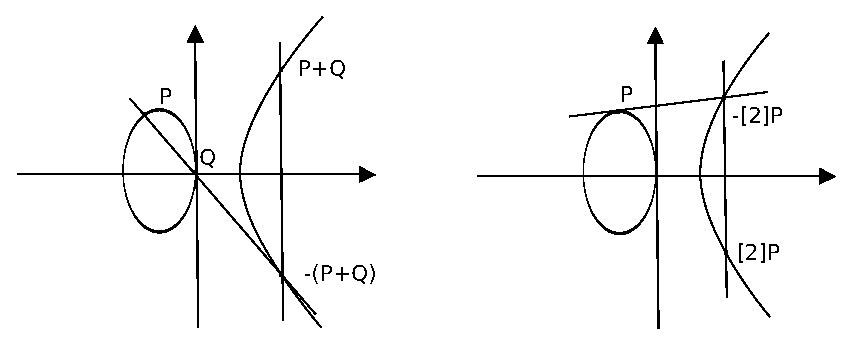
\includegraphics[scale=1]{./images/Group_law_of_ECC}
  \caption{The group law on elliptic curve. Adapted from \cite{Cohen}.}\label{EC}
\end{figure}

To illustrate the group law, $P$ and $Q$ are two points on the curve,
a third point can be made which is the intersection of the curve with
a line through $P$ and $Q$ (the left in Figure \ref{EC}). $P\oplus Q$
is given by mirroring the intersection point at the
$x$-axis. Furthermore, the sum of two points with the same
$x$-coordinate needs to be calculated (the right in Figure
\ref{EC}). A "point at infinity" $P_\infty$ is defined, it can be
understood as any line, which is parallel to the $y$-axis. This point
is the neutral point of the group, so that
$(x_1,y_1)\oplus(x_1,-y_1)=P_\infty$, i.e., $(x_1,-y_1)=-P$.

\hhline

In the ACL three types of elliptic curves are supported:
\begin{itemize}
\item $y^2 \equiv x^3 + Ax + B$ mod $p$ with $p \in \textbf{P} \setminus \{2,3\}$\\
      It is defined over the finite field $F_p$. (Section \ref{ZP})
\item $y^2 + xy \equiv x^3 + Ax^2 + B$ mod $f(z)$\\
      It is defined over the binary field $GF(2^{deg(f)})$. (Section \ref{NSS})\\
      \textbf{Precondition:} $f(z)$ is an irreducible polynomial.
\item $y^2 + Cy \equiv x^3 + Ax + B$ mod $f(z)$\\
      It defines supersingular elliptic curves over the binary field $GF(2^{deg(f)})$. (Section \ref{SS})\\
      \textbf{Precondition:} $f(z)$ is an irreducible polynomial.
\end{itemize}

%%%%%%%%%%%%%%%%%%%%%%%%%%%%%%%%%%%%%%%%%%%%%%%%%%%%%%%%%%%%%%%%%%%%%%%%%%%
%%%%%%%%%%%%%%%%%%%%%%%%%%%%%%%%%%%%%%%%%%%%%%%%%%%%%%%%%%%%%%%%%%%%%%%%%%%

\section{Root Package: Crypto.Types.Elliptic\_Curves}\label{EllipticRoot}
It is the root package of the elliptic curves. A basic type \texttt{EC\_Point} is defined for all three elliptic curve types.
\subsubsection*{Generic Part}
\begin{lstlisting}{}
  generic
  	with package Big is new Crypto.Types.Big_Numbers(<>);
\end{lstlisting}
\subsubsection*{Types}
The global type \texttt{EC\_Point} is defined.
\begin{lstlisting}{}
   -- (x,y)
  type EC_Point is record
  	 X : Big.Big_Unsigned;
    Y : Big.Big_Unsigned;
  end record;
  EC_Point_Infinity : constant EC_Point;
\end{lstlisting}
The constant \texttt{EC\_Point\_Infinity} of type \texttt{EC\_Point}
equals $\infty$. This point is located on each elliptic curve and
corresponds to the neutral element of addition.

%%%%%%%%%%%%%%%%%%%%%%%%%%%%%%%%%%%%%%%%%%%%%%%%%%%%%%%%%%%%%%%%

\subsubsection*{Procedures}
\begin{lstlisting}{}
  procedure Put(Item: in EC_Point, Base: in Number_Base := 10);
  procedure Put_Line( Item : in EC_Point, 
                      Base : in Number_Base := 10);
\end{lstlisting}
These two procedures output a \texttt{EC\_Point} in the standard output form of a tupel.\\

\noindent\textbf{Example:}
\begin{lstlisting}{}
  procedure Example_EC is
    P: EC_Point(X => Big_Unsigned_Three, Y => Big_Unsigned_One);
  begin
    Put(P);             -- Output: "(3,1)"
    Put(P, Base => 2);  -- Output: "(2#11#, 2#1#)"
  end Example_EC;
\end{lstlisting}

%%%%%%%%%%%%%%%%%%%%%%%%%%%%%%%%%%%%%%%%%%%%%%%%%%%%%%%%%%%%%%%%
%%%%%%%%%%%%%%%%%%%%%%%%%%%%%%%%%%%%%%%%%%%%%%%%%%%%%%%%%%%%%%%%

\section{Child Packages}
There are three child packages of the \texttt{Crypto.Types.Elliptic\_Curves}:
\begin{itemize}
\item \texttt{Crypto.Types.Elliptic\_Curves.Zp} \\
      -- elliptic curves over finite fields
\item \texttt{Crypto.Types.Elliptic\_Curves.NSS\_BF}\\
      -- non-supersingular elliptic curves over binary fields
\item \texttt{Crypto.Types.Elliptic\_Curves.SS\_BF}\\
      -- supersingular elliptic curves over binary fields
\end{itemize}
%implement each elliptic curves introduced above.
\subsection{Elliptic\_Curves.Zp}\label{ZP}
It implements an elliptic curve over a finite field $Z_p$.
\subsubsection*{Types}
In the package a variable type \texttt{Elliptic\_Curve\_Zp} is defined. It is only used in domain of this package.
\begin{lstlisting}{}
  --(A,B,P)
  type Elliptic_Curve_Zp is record
	 A : Big_Unsigned;
	 B : Big_Unsigned;
	 P : Big_Unsigned;
  end record;
\end{lstlisting}
$A,B,P$ are coefficients according to $y^2 \equiv x^3 + Ax + B$ mod $p$.
\subsubsection*{API}
\begin{lstlisting}{}
  procedure Init(A, B, P : in Big_Unsigned);
  procedure Init(ECZ     : in Elliptic_Curve_Zp);
  procedure Init(Len     : in Positive);
\end{lstlisting}
These are three ways to initialize the elliptic curves.  $A,B,P$ are
three compositions of the type \texttt{Elliptic\_Curve\_Zp}. The first
two procedures assign the parameters with delivered values. In the
third procedure, it searches prime numbers within the delivered bit
length and then initialises all variables.

These procedures make just an assignment or an initialization. Whether
the curve is an elliptic curve or not, can be tested by other
functions within the package.\\ 

\noindent\textbf{Exception:} If the
\texttt{Len} $<$ 3:\quad\texttt{Constraint\_Error}.

\hhline
\begin{lstlisting}{}
  function Is_Elliptic_Curve return Boolean;
\end{lstlisting}
This function tests whether the curve is an elliptic curve or not.
$P$ must be a prime number bigger than 3, and the discriminant of the
curve: $\bigtriangleup = -16(4a^3+27b^2)$ must be nonzero. It returns
true, if the curve meets the two requirements. When it fails, the
remaining functions may not return the desired results.

\hhline

\begin{lstlisting}{}
  function On_Elliptic_Curve(X : EC_Point) return Boolean;
\end{lstlisting}
This function tests, whether a point $X$ is on the elliptic curve or
not. In the situation that $X$ equals \texttt{EC\_Point\_Infinity},
the function returns true.

\hhline

\begin{lstlisting}{}
  function Negative   (X : EC_Point)           return EC_Point;
  function Is_Negative(X : EC_Point)           return Boolean;
  function Is_Negative(Left, Right : EC_Point) return Boolean;
\end{lstlisting}
The function \texttt{Negative()} returns the value $-X$.\\ The
function \texttt{Is\_Negative()} with parameter $X$ tests if $X$
equals \texttt{EC\_Point\_Infinity} or if $-X$ equals
\texttt{Big\_Unsigned\_Zero}. It returns true if one of the two
situations happens.\\ The last function test if both \texttt{Left} and
\texttt{Right} equal \texttt{EC\_Point\_Infinity}, or whether
\texttt{Left} is the negative of \texttt{Right}.

\hhline

\begin{lstlisting}{}
  function "+"(Left, Right : EC_Point) return EC_Point;
  function "-"(Left, Right : EC_Point) return EC_Point;
  function "*"(Left  : Big_Unsigned; Right : EC_Point) return EC_Point;
\end{lstlisting}
Here the basic operations for variables of \texttt{EC\_Point} are defined.

\hhline

\begin{lstlisting}{}
  function Double(X : EC_Point) return EC_Point;
\end{lstlisting}
This function calculates $2X$.\\

%%%%%%%%%%%%%%%%%%%%%%%%%%%%%%%%%%%%%%%%%%%%%%%%%%%%%%%%%%%%%%%%%

\subsection{Elliptic\_Curves.NSS\_BF}\label{NSS}
In this package the elliptic curve $y^2 + xy \equiv x^3 + Ax^2 + B$
mod $f(z)$ is implemented. Some commen operations have been already
introduced in \texttt{Crypto.Types.Elliptic\_Curves.Zp}, Section
\ref{ZP} can be refered for details.
\subsubsection*{API}
\begin{lstlisting}{}
  procedure Init(A, B, F : in Big_Unsigned);
\end{lstlisting}
The procedure makes the initialization. $A,B$ are two coefficients,
and $F$ is a polynomial that creates the binary field
$GF(2^{deg(F)})$.

\hhline

\begin{lstlisting}{}
  function Is_Elliptic_Curve return Boolean;
\end{lstlisting}
The funtion tests if the curve after the initialization is a valid
elliptic curve or not. It tests if F is irreducibel, and computes if
the discriminant of the elliptic curve is nonzero. Unfortunately the
test of $F$ is still in plan.\\
\subsection{Elliptic\_Curves.SS\_BF}\label{SS}
This package implements the elliptic curve $y^2 + Cy = x^3 + Ax + B$
mod $f(z)$. Some commen operations have been already introduced in
\texttt{Crypto.Types.Elliptic\_Curves.Zp}, Section \ref{ZP} can be
refered for details.
\subsubsection*{API}
\begin{lstlisting}{}
  procedure Init(A, B, C, F : in Big_Unsigned);
\end{lstlisting}
$A,B,C$ are the coefficients of the curve, and $F$ is a polynomial
that creates the binary field $GF(2^{deg(F)})$.

\hhline

\begin{lstlisting}{}
  function Is_Elliptic_Curve return Boolean;
\end{lstlisting}
It tests if the curve after the initialization is a valid elliptic
curve or not. It tests if F is irreducibel, and computes if the
discriminant of the elliptic curve is nonzero. Unfortunately the test
of $F$ is still in plan.\\
\subsection{Elliptic Curves Database $Z_p$}
One elliptic curves database of this form
\begin{itemize}
\item $y^2 = x^3 + Ax + B$ mod $p$ with $p \in \textbf{P} \setminus \{2,3\}$ \\
      -- elliptic curve defined over the finite field $Z_p$.
\end{itemize}
is provided in the ACL, which contains the elliptic curves published
by NIST (National Institute of Standards and Technology). The
following curves are included: 
\begin{center}
Curve P-192/244/384/521 and Test Curve (5-bit).
\end{center}


\subsubsection*{Generic Part}
\begin{lstlisting}{}
  package Elliptic_Curve_Database_Map is
      new Ada.Containers.Ordered_Maps (Key_Type => Bit_Length,
                   Element_Type => Precomputed_Elliptic_Curve);
\end{lstlisting}
\subsubsection*{Types}
This package defines two types: \texttt{Bit\_Length} and \texttt{Precomputed\_Elliptic\_Curve}.
\begin{lstlisting}{}
  type Bit_Length is new natural;
  type Precomputed_Elliptic_Curve is record
    P : String(1..192) := (others=>' ');   -- prime modulus
    R : String(1..192) := (others=>' ');   -- order
    S : String(1..192) := (others=>' ');   -- 160-bit input seed to SHA-1
    C : String(1..192) := (others=>' ');   -- output of SHA-1
    B : String(1..192) := (others=>' ');   -- coefficient b
    Gx : String(1..192) := (others=>' ');  -- base point x coordinate
    Gy : String(1..192) := (others=>' ');  -- base point y coordinate
    length : Bit_Length;	           -- bit length
  end record;
\end{lstlisting}
\subsubsection*{Procedures}
\begin{lstlisting}{}
  procedure Get_Elliptic_Curve(ECZ    : out Elliptic_Curve_Zp;
                               ECP    : out EC_Point;
                               order  : out Big_Unsigned;
                               length : in  Bit_Length);
\end{lstlisting}
This procedure takes related variables from the database, which are
required to compute an elliptic curve. The curve has at least a
cryptographic security in \texttt{length}. \\

\noindent\textbf{Exception:} The
\texttt{length} has a range from 0 to 521 bits (max. bit length = 521
bits). If a \texttt{length} value is not
included:\quad\texttt{LEN\_ERROR}.\\

\noindent\textbf{Example:}
\begin{lstlisting}{}
  with Crypto.Types; use Crypto.Types;
  with Crypto.Types.Big_Numbers;
  with Crypto.Types.Elliptic_Curves.Zp;
  with Crypto.Types.Elliptic_Curves.Zp.Database;

  procedure Example_EC_DB_ZP is
    package Big is new Crypto.Types.Big_Numbers(Size);
    use Big;
    package EC is new Crypto.Types.Elliptic_Curves(Big);
    use EC;
    package Zp is new EC.Zp;
    use Zp;
    package DB is new Zp.Database;
    use DB;
    EC_ZP : Elliptic_Curve_Zp;
    EC_P  : EC_Point;
    order : Big_Unsigned;
  begin
    Get_Elliptic_Curve(EC_ZP, EC_P, order, 168);
  end Example_EC_DB_ZP;
\end{lstlisting}
